\section{Problems}

\subsection{[Basic Statistics]}

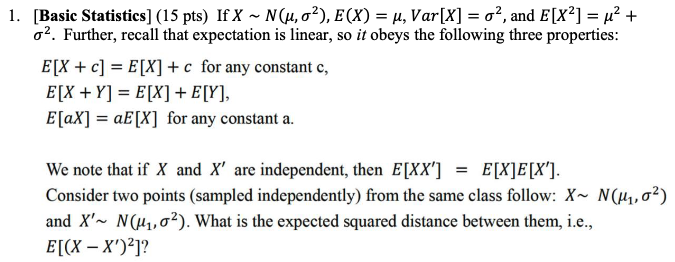
\includegraphics[width=1\textwidth]{media/hw2_q1.png}

\subsection{[Basic Linear Algebra] (15 pts) We are given a vector $x = [0, 0.2, 1.0, 2.2]$. Which of the following vector is closest to $x$ and what is the distance from the closest point to $x$ under each of the following vector norms?}

$$x_1 = [0.7, 0.2, 0.5, 2.0]$$
$$x_2 = [0, 1.0, 1.5, 2.2]$$
$$x_3 = [0.8, 0.1, 1.2, 2.0]$$

a) 0-norm =
b) 1-norm =
c) 2-norm =
d) $\infty$-norm =

\subsubsection{For $\mathbf{x_1}$:}
\begin{align}
    ||\mathbf{x} - \mathbf{x_1}|| &= 
    \begin{bmatrix}
        |0 - 0.7| & |0.2 - 0.2| & |1 - 0.5| & |2.2 - 2|
    \end{bmatrix} \nonumber \\
    &= 
    \begin{bmatrix}
        0.7 & 0 & 0.5 & 0.2
    \end{bmatrix} 
\end{align}
\begin{align}
    \Rightarrow ||\mathbf{x_1}||_0 &= 3
\end{align}
\begin{align}
    \Rightarrow  ||\mathbf{x_1}||_1 &= \sum ||\mathbf{x} - \mathbf{x_1}|| = 0.7 + 0 + 0.5 + 0.2 = 1.4
\end{align}
\begin{align}
    \Rightarrow ||\mathbf{x_1}||_2 &= \sqrt{|0 - 0.7|^2 + |0.2 - 0.2|^2 + |1 - 0.5|^2 + |2.2 - 2|^2} \nonumber \\
    &= \sqrt{0.7^2 + 0^2 + 0.5^2 + 0.2^2} = \sqrt{0.78} = 0.8832
\end{align}
\begin{align}
    \Rightarrow ||\mathbf{x_1}||_{\infty} &= max ||\mathbf{x} - \mathbf{x_1}|| = 0.7
\end{align}

\subsubsection{For $\mathbf{x_2}$:}
\begin{align}
    ||\mathbf{x} - \mathbf{x_2}|| &= 
    \begin{bmatrix}
        |0 - 0| & |0.2 - 1| & |1 - 1.5| & |2.2 - 2.2|
    \end{bmatrix} \nonumber \\
    &= 
    \begin{bmatrix}
        0 & 0.8 & 0.5 & 0
    \end{bmatrix} 
\end{align}
\begin{align}
    \Rightarrow ||\mathbf{x_2}||_0 &= 2
\end{align}
\begin{align}
    \Rightarrow  ||\mathbf{x_2}||_1 &= \sum ||\mathbf{x} - \mathbf{x_2}|| = 0 + 0.8 + 0.5 + 0 = 1.3
\end{align}
\begin{align}
    \Rightarrow ||\mathbf{x_2}||_2 &= \sqrt{|0 - 0|^2 + |0.2 - 1|^2 + |1 - 1.5|^2 + |2.2 - 2.2|^2} \nonumber \\
    &= \sqrt{0^2 + 0.8^2 + 0.5^2 + 0^2} = \sqrt{0.89} = 0.9434
\end{align}
\begin{align}
    \Rightarrow ||\mathbf{x_2}||_{\infty} &= max ||\mathbf{x} - \mathbf{x_2}|| = 0.8
\end{align}

\subsubsection{For $\mathbf{x_3}$:}
\begin{align}
    ||\mathbf{x} - \mathbf{x_3}|| &= 
    \begin{bmatrix}
        |0 - 0.8| & |0.2 - 0.1| & |1 - 1.2| & |2.2 - 2|
    \end{bmatrix} \nonumber \\
    &= 
    \begin{bmatrix}
        0.8 & 0.1 & 0.2 & 0.2
    \end{bmatrix} 
\end{align}
\begin{align}
    \Rightarrow ||\mathbf{x_3}||_0 &= 4
\end{align}
\begin{align}
    \Rightarrow  ||\mathbf{x_3}||_1 &= \sum ||\mathbf{x} - \mathbf{x_2}|| = 0.8 + 0.1 + 0.2 + 0.2 = 1.3
\end{align}
\begin{align}
    \Rightarrow ||\mathbf{x_3}||_2 &= \sqrt{|0 - 0.8|^2 + |0.2 - 0.1|^2 + |1 - 1.2|^2 + |2.2 - 2|^2} \nonumber \\
    &= \sqrt{0.8^2 + 0.1^2 + 0.2^2 + 0.2^2} = \sqrt{0.73} = 0.8544
\end{align}
\begin{align}
    \Rightarrow ||\mathbf{x_3}||_{\infty} &= max ||\mathbf{x} - \mathbf{x_3}|| = 0.8
\end{align}

Based on the above norm calculations, we have the following results:
\begin{enumerate}
    \item by the 0-norm, $\mathbf{x_2}$ is the closest to $\mathbf{x}$.
    \item by the 1-norm, both $\mathbf{x_2}$ and $\mathbf{x_3}$ are the closest to $\mathbf{x}$.
    \item by the 2-norm, $\mathbf{x_3}$ is the closest to $\mathbf{x}$.
    \item by the $\infty$-norm, $\mathbf{x_1}$ is the closest to $\mathbf{x}$.
\end{enumerate}

\subsection{[Convexity] (1)}

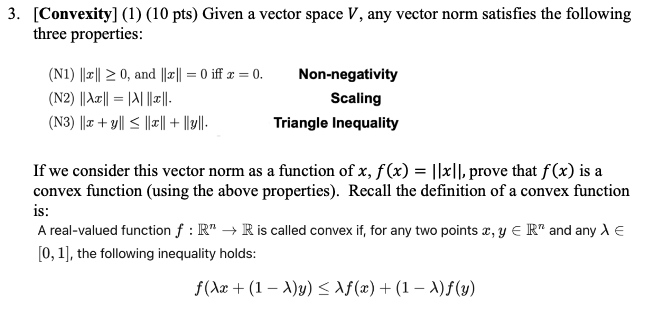
\includegraphics[width=1\textwidth]{media/hw2_q3.png}

\subsection{[Convexity] (2) (10 pts). Prove that the convexity is preserved under a linear transformation. Supposed $f(w)$ is convex in terms of $w$. Prove that $g(w)=f(X w + b)$ is also convex in terms of $w$ where $X$ is a fixed matrix of appropriate size, and $b$ is a fixed vector of appropriate size. (So $X$ and $b$ are not variables in $g$). (Hint: you can simply use the definition of convex function)}

\subsection{[Convexity] (3) (10 pts). From (1) and (2), prove the “loss” function $||y-Xw||_2$ is convex in terms of $w$ where $X_{n \times d}$ is a data matrix containing $n$ examples and each example has $d$ features, and $y$ is a column vector of length $d$. This dataset has been observed and thus fixed, and $w$ is the only variable in the norm.}